\documentclass[conference,10pt,letterpaper,twoside]{ieeeconf}

\IEEEoverridecommandlockouts

% to use ieeeconf with natbib
\makeatletter
\let\NAT@parse\undefined
\makeatother

\usepackage[numbers,sort,compress]{natbib}

\usepackage{graphicx}
\usepackage{color}
\usepackage{multirow}
\usepackage{balance}

\usepackage{amsmath,amssymb} % define this before the line numbering.
\usepackage{mathtools}
\usepackage{algorithmic}
\usepackage{algorithm}

\usepackage{caption}
%\usepackage[skip=0pt]{subcaption}
\usepackage{subcaption}
\captionsetup{
   labelfont = small,%footnotesize,
   textfont = small,%footnotesize,
   %skip = 1ex,  % skip the space between float and caption
   %belowskip=-10pt,
}

% perls packages
\usepackage{perl_acronyms}
\usepackage{perl_math}
\usepackage{perl_SIunits}
\usepackage{perl_misc}


\definecolor{ared}{RGB}{255,0,0}
\newcommand{\aku}[1]{{\color{ared}[aku:}\ {\color{ared}#1]}}

\definecolor{jgreen}{RGB}{0,155,0}
\newcommand{\jmw}[1]{{\color{jgreen}[jmw:\ #1]}}


\title{Towards Generating Probabilistic Object Detection Maps}

\author{Arash~K.~Ushani, Ryan~W.~Wolcott, Jeffrey~M.~Walls, and Ryan~M.~Eustice%
   \thanks{This work was supported by a grant from the Toyota Research Institute under
       award N021515.}
   \thanks{A.~Ushani and R.~Eustice are with the University of Michigan, Ann Arbor,
       MI 48109, USA.
       \texttt{\{aushani, eustice\}@umich.edu}.}
   \thanks{R.~Wolcott and J.~Walls are with the Toyota Research Institute.
    \texttt{\{rwolcott, jmwalls\}@umich.edu}.}%
}


\begin{document}

\maketitle

\begin{abstract}
%
Estimating the pose of visible and occluded objects in the environment is a core
competency for autonomous robotic systems. Standard object detection pipelines
typically report a list of object locations per class, but do not directly
support reasoning about where objects \emph{could} be. In this work, we work
towards augmenting the state-of-the-art LIDAR detection algorithms with a notion
of free and unknown space. Importantly, this distinction enables computing a
distribution over per class object locations, which allows reasoning about
anywhere in the immediate environment, including into occluded regions. We
evaluate our method on the publicly available KITTI dataset.
%
\end{abstract}

\acresetall

%\IEEEpeerreviewmaketitle

\acused{GPU}

\section{Introduction}\label{sec:intro}

A core competency of many autonomous systems is to be aware of the state of
their environments so that they may operate safely in them. For example, an
autonomous vehicle needs to be aware of other cars on the road for a path
planning module to propose safe actions. This object detection task has been
extensively studied in the literature using different sensor modalities,
including camera imagery and \ac{LIDAR}.

However, object detection alone does not paint a complete picture of the
environment for the robot. It is also critical for a robot to make inferences
and decisions regarding where objects possibly \emph{could} be; for example, a
robot might need to ask ``how likely is it that a pedestrian is present in this
occluded region?" The answer to this question can be the difference between
driving through an intersection unhindered or cautiously anticipating a
pedestrian hidden behind a parked car.

\begin{figure}[!t]
  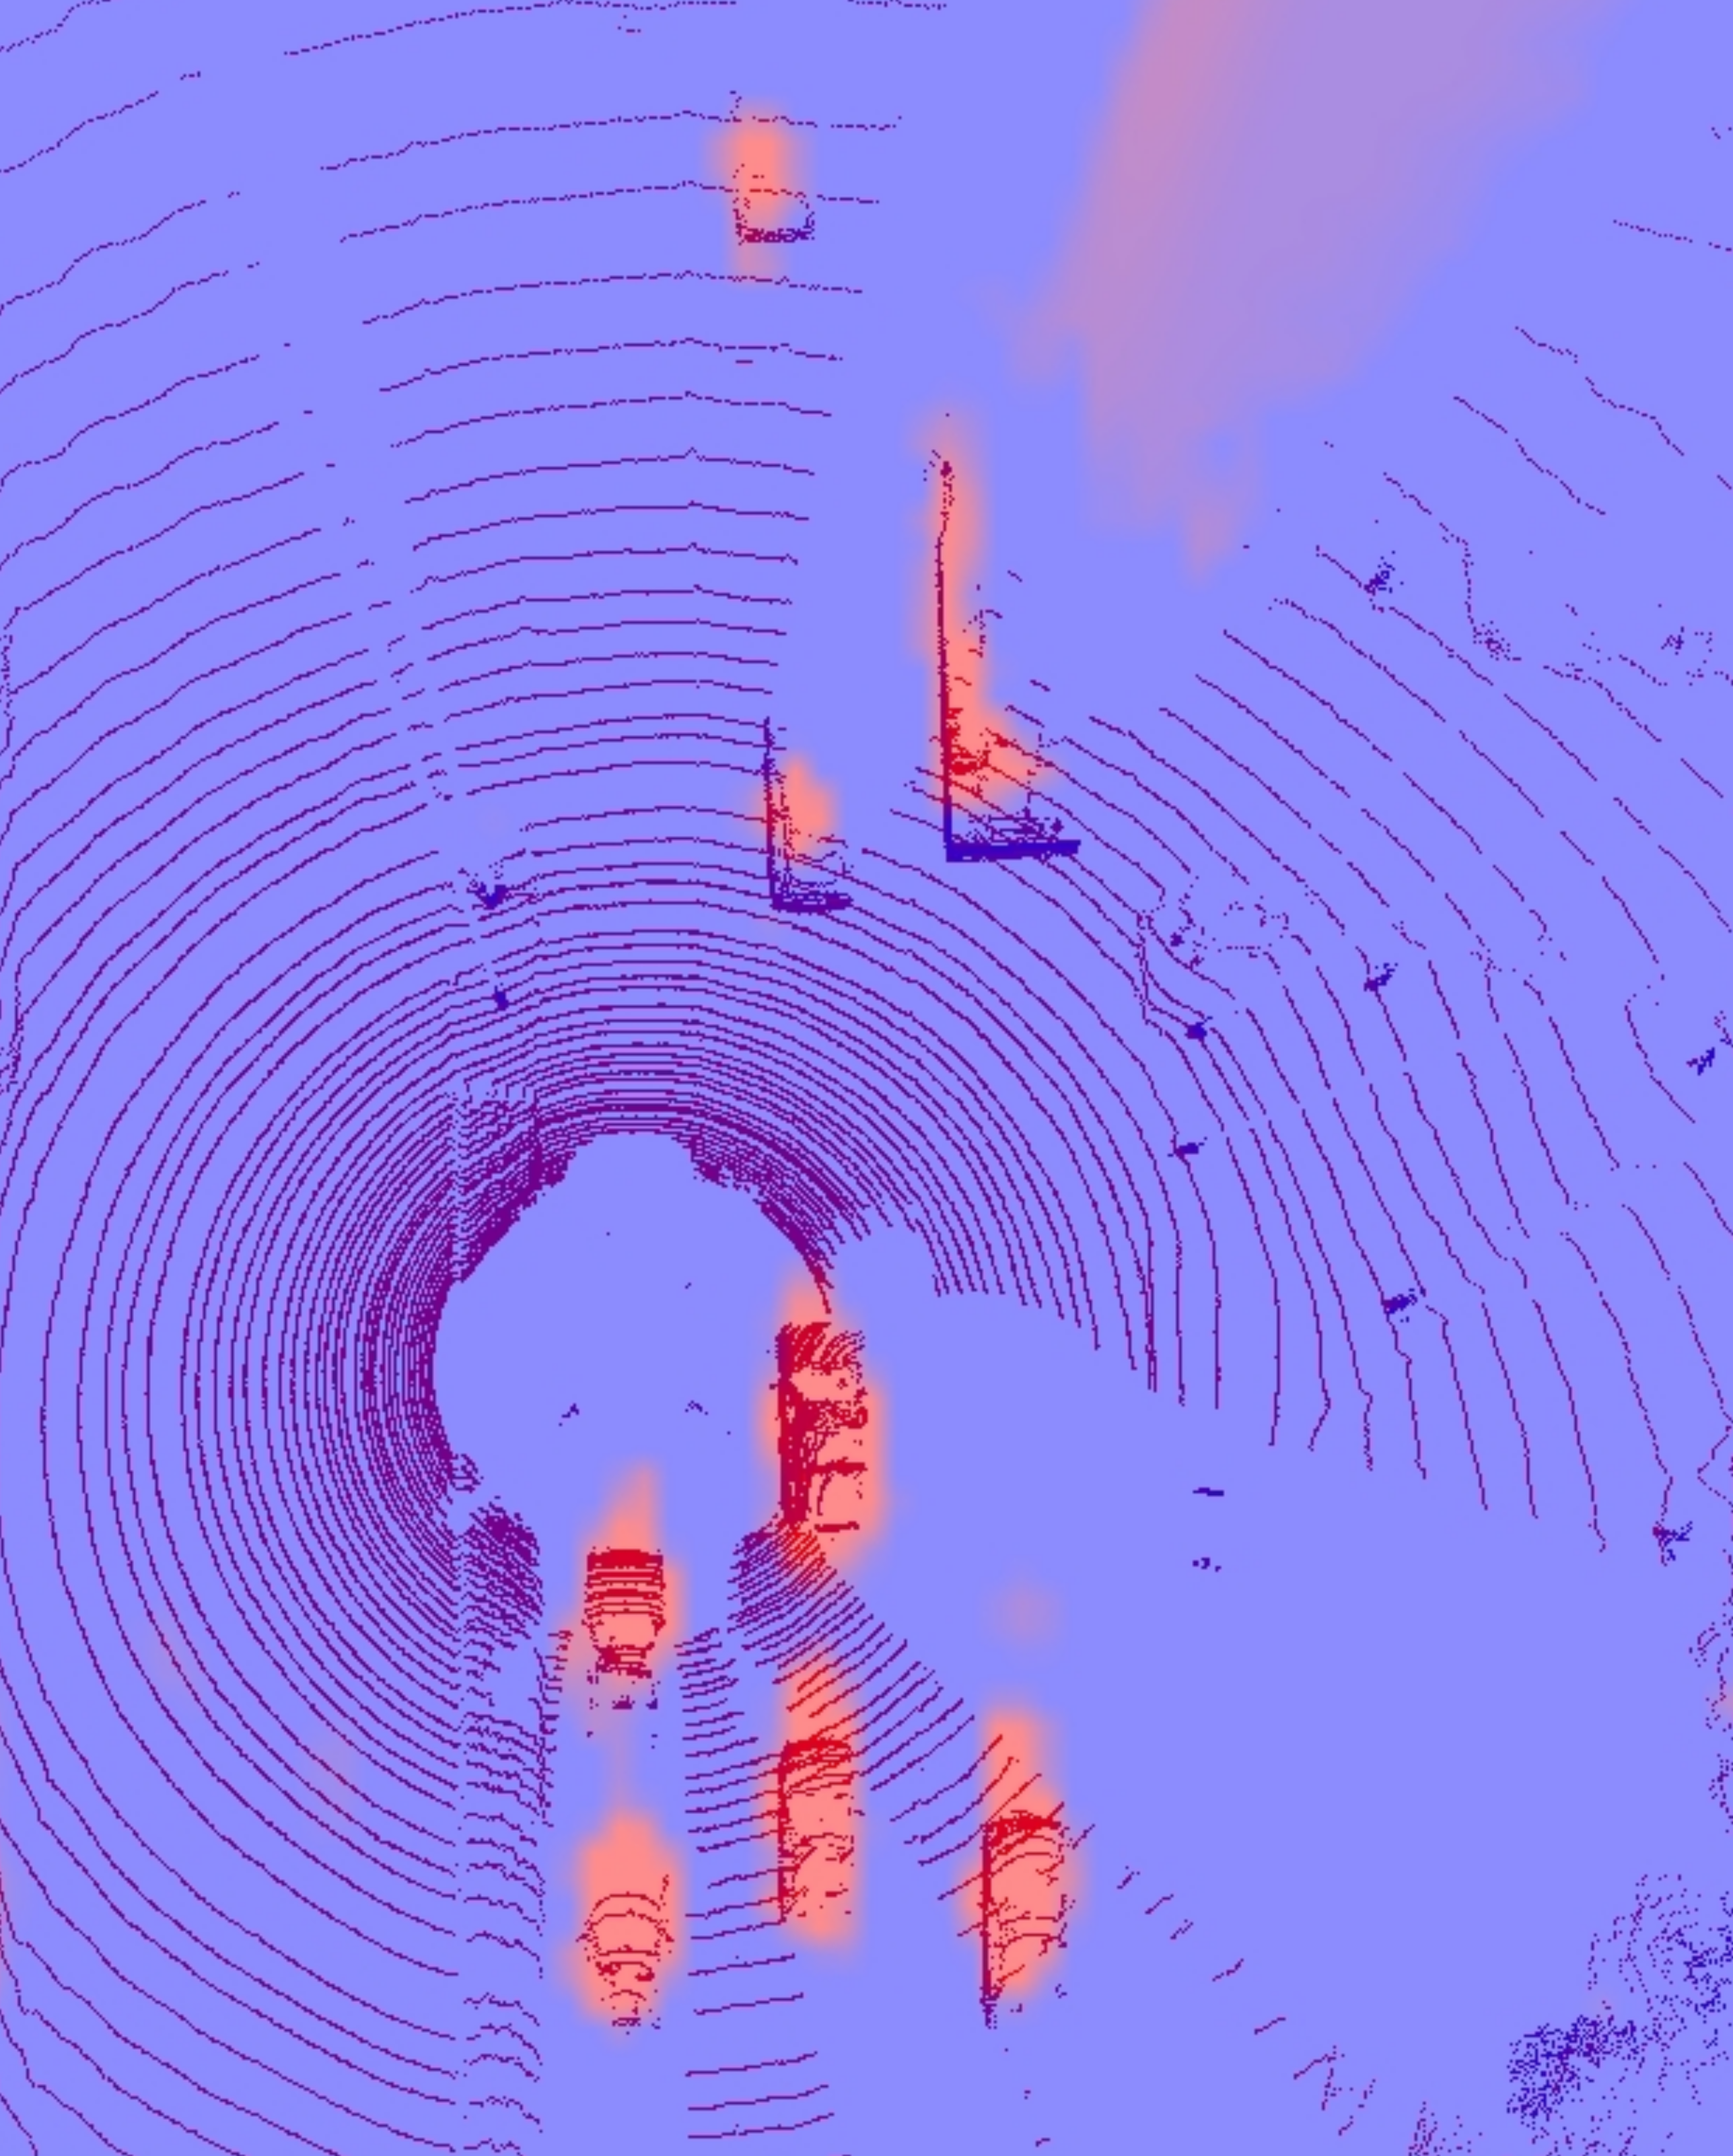
\includegraphics[width=\columnwidth]{figures/badge.jpg}
  \caption{A bird's eye view of sample output from our proposed system run on
    the KITTI dataset. Red colors indicate high probabilities for cars, blue
    indicates high probabilities for background. (Best viewed in color.) }
  \vspace{-7mm}
  \label{fig:badge}
\end{figure}

\figref{fig:badge} shows an example of a situation that an autonomous car might
encounter. In addition to detecting the cars present in the environment, we
wish to capture areas we know are absent of cars (shown in blue) or areas where
there might be cars that are hidden (such as the occluded region in the top
right).

The state-of-the-art in object detection, while performing very well in the pure
detection task, is ill-suited to answer these types of queries. These methods
typically do not fully model the nature of range-based sensors such as
\ac{LIDAR}, often using solely the points that are returned. Thus, there is no
way to differentiate between free and unknown regions of the world.

Occupancy mapping and related work is better suited for differentiating between
free and unknown space, as they explicitly model these. However, this mapping is
typically performed per voxel, and there is no notion of the potential absence
or presence of an \emph{object class}.

In this paper, we blend these two paradigms; we present a method that
consumes \ac{LIDAR} data and produces a probabilistic distribution of object-level
detections that can represent known objects in the world, areas were objects are
known to be absent, and regions of uncertainty. To achieve this, we rely on
techniques from both approaches, including ray-casting to sweep out free space
and the use of object-level observation models. Additionally, we formulate our
approach in a Bayesian framework, allowing for simple integration of additional
sensor modalities.

The goals of this work include:
%
\begin{itemize}
  \item Explicitly modeling occupied, free, and unknown space in a Bayesian
    formulation that is easily amendable to multi-modal sensing or temporal
    updates.
  \item Generation of a probabilistic detection map that can be queried at any
    location for the presence of a given object.
\end{itemize}
%
Additionally, we provide some preliminary results of this approach on the KITTI
dataset \cite{Geiger2013IJRR}.

\section{Related Work}\label{sec:rw}

There is a rich literature in both object-level detection and probabilistic
mapping. In object detection, many methods can be regarded as simply taking some
kind of object classifier and applying it to locations in the environment. These
locations can either be searched exhaustively or by some guided method, such as
segmentation or region proposal. \citet{wang2012could} segmented and clustered a
laser scan before classifying each segment according to background or foreground
object. \citet{wang2015RSS} implemented a sliding window SVM detector with a
voting scheme that allowed for efficient processing of sparse \ac{LIDAR} data.
Building upon this idea, \citet{Engelcke2017ICRA} showed that this same voting
scheme could be adapted for use with a \ac{CNN}.

Another approach is to process all of the sensor data together. In one of the
earlier works, \citet{petrovskaya-2009} created virtual 2D scans from \ac{LIDAR}
data and used a Bayes filter per object to estimate both the dynamics and simple
geometries properties, such as width and length. This filter is then maintained
over time as more observations are made. More recently, this type of approach has
been popular in a deep learning approach using camera data
\citep{yang2016exploit, deepmanta_cvpr17, Ren17CVPR}, but has also been applied
to \ac{LIDAR} sensor data as well. \citet{Li2016RSS} process a range image from
a \ac{LIDAR} sensor using a \ac{FCN} to generate bounding boxes for car
detections. \citet{Chen2017CVPR} build a fusion network that takes as input both
camera imagery and also multiple views of a \ac{LIDAR} point cloud, such as a
bird's eye view or a front view. However, these approaches do not explicitly model
the notion of free space and occluded regions.

Occupancy mapping \cite{thrun2005probabilistic} and its derivatives (such as
\cite{hornung13auro}) are commonly used to model the full
information captured by a range sensor such as \ac{LIDAR}, properly modeling
free and occluded space while also representing unknown areas at the level of discrete
voxels. \citet{gpmaps_ijrr12} introduced Gaussian process occupancy maps, a
technique that exploits the structure of environments (e.g., the occupancy of
some position in the world is correlated with its neighborhood). More recently,
\citet{Ramos-RSS-15} introduced Hilbert mapping, a somewhat related approach in
which a kernelized logistic regression is trained to predict occupied or free
space from online sensor measurements. Extensions of this framework explored how
to leverage the choice of kernels used in the regression, essentially modeling
features that capture structure primitives \citep{Guizilini-RSS-17,
  guizilini2016large}. However, these approaches do not focus on capturing
specific object classes.

Recently, there has been some work in object detection and classification from
occupancy grids or similar representations, typically using some kind of
volumetric or multiview \ac{CNN} \cite{qi2016volumetric, maturana2015voxnet}.
These methods tend to do well with occlusions, as evidenced by the
performance of similar techniques in shape completion \cite{smith2017CORL,
  dai2017complete}. However, these approaches focus on classify a single
instances of an object from a single occupancy grid or similar representation.
As such, it is intractable to scale them into an exhaustive search.

Our work lies at the intersection of object detection and occupancy mapping. We
propose a representation that provides the benefits of both approaches, namely,
understanding at an object level and capturing both known and unknown areas.


\section{Problem Setup}

Consider a set of LIDAR observations $\mathbf{Z} = \{ z_i \}_{i=1}^n$, where
each $z_i$ represents a ray at angle $\theta_i$ with range $r_i$. We
want to evaluate
%
\begin{align}
  p( obj_c | \mathbf{Z} )
  \text{,}
\end{align}
%
where $obj_c$ represents an object of class $c$ that exists at some position $(x,
y)$ and at some angle $\theta_{\text{object}}$. For this experiment, we will use
stars and boxes of variable size as our objects. Additionally, we model $p(
obj_{\text{no obj.}} | \mathbf{Z})$, the probability that no object exists at $(x,
y)$.

Using Bayes' rule and assuming conditionally independent observations given the
object, we have:
%
\begin{align}
  p( obj_c | \mathbf{Z} ) &= \frac{p(\mathbf{Z} | obj_c) p(obj_c)}{p(\mathbf{Z})} \\
    &= \frac{p(obj_c) \prod_{i=1}^{n} { p( z_i | obj_c) }} {p(\mathbf{Z})}
    \label{eq:cond_ind}
  \text{.}
\end{align}
%
Taking the log probability, we have:
%
\begin{align}
  \log p( obj_c | \mathbf{Z} ) &= \log{\eta} + \sum_{i=1}^{n} { \log p( z_i |
    obj_c) } + \log p ( obj_c )
  \text{,}
  \label{eq:obj_model}
\end{align}
%
where $\eta = \frac{1}{p(\mathbf{Z})}$ is a normalization constant.

\section{Method} \label{sec:method}

We investigate several different ways to evaluate the observation model.

\subsection{Ray-Based}

In \cite{ushani_raybased}, we extensively studied how to evaluate the
observation by using a ray-based approach. Each observation $z_i$ is modeled as
a ray from the sensor origin to the point return (thus capturing the free space
between the sensor and the returned point). We built a ray-based observation
model for each object class using a discretized lookup table of histograms that
were learned during training. Additionally, to improve performance when dealing
with multiple classes, the conditional dependence of $z_i$ on $z_{i-1}$ was
modeled as well. While this approach showed promising results in a 2D simulated
world, it was intractable to scale up to 3D, with the chief problem being
training a higher dimensional observation model.

\subsection{Occupancy Grid}

To make the problem more tractable in 3D, we considered building an occupancy
grid from the \ac{LIDAR} observations $\mathbf{Z}$. This occupancy grid consists
of a sparse set of voxels $\mathbf{V} = \{v_{1:n_v}\}$, where each voxel $v_i$
is labeled as either free or occupied. Any voxels not contained in this sparse
set is considered to be unknown. We compute $\mathbf{V}$ by performing
ray-casting using Bresenham's ray tracing algorithm
\cite{bresenham1965algorithm}. This can be efficiently implemented on a \ac{GPU}

Thus, for our observation model, we now wish to evaluate:
%
\begin{align}
  p(\mathbf{V} | \mathrm{obj_{c, x}}) \text{.} \label{eq:detection_map}
\end{align}

\subsubsection{Na\"ive Bayes} \label{sec:naive_bayes}

One approach is to make the independence assumption:
%
\begin{align}
  p(\mathbf{V} | \mathrm{obj_{c, x}}) &= \prod_i p(v_i | \mathrm{obj_{c, x}})
  \text{.}
\end{align}
%
The key advantage of this approach is its simplicity and speed.
However, we find that this assumption leads to significant confusion between
classes. As each voxel is assumed to be independent given the presence of an
object, this model does not capture any of the dependencies between voxels in
the case in intra-class variation, leading to degradation in performance. For
example, this model cannot easily distinguish between a car and a bush that is
roughly the same size as a car.

\subsubsection{Chow-Liu Tree Model} \label{sec:clt}

Similar to our work in \cite{ushani_raybased}, we propose better approximating
the full joint distribution $p(\mathbf{V} | \mathrm{obj_{c,x}})$ by modeling
some of the conditional dependence between observations. To do so, we leverage a
\ac{CLT} \citep{chow1968approximating}.

For the observations $\mathbf{V} = \{v_1, \ldots, v_{n_z}\}$, a \ac{CLT} finds a
first order dependency tree between them that minimizes the \ac{KLD} between the
approximated distribution $P$ and the true full joint distribution $Q$:
%
\begin{align}
  D(P || Q) &= -\sum I(v_i, v_{p(i)}) + \sum H(v_i) - H(\mathbf{V})
  \label{eq:kld}
  \text{,}
\end{align}
%
where $I(v_i, v_{p(i)})$ is the mutual information between $v_i$ and its parent
in the tree $v_{p(i)}$, $H(v_i)$ is the entropy of $v_i$, and $H(\mathbf{V})$ is
the joint entropy of $\{v_1, \ldots, v_{n_z}\}$. To minimize the \ac{KLD}, the
\ac{CLT} finds the spanning tree amongst $\mathbf{V}$ that maximizes the total
pairwise mutual information, as the latter two terms in \eqref{eq:kld} are
independent of the dependency tree's structure.

To evaluate the \ac{CLT} approximation of the distribution, we compute:
%
\begin{align}
  p(\mathbf{V)} &\approx p_{clt}(\mathbf{V}) = p(v_r) \prod p(v_i | v_{p(i)})
\end{align}
%
where $v_r$ is the voxel chosen as the root of the spanning tree.

\subsubsection{Greedy CLT Approximation} \label{sec:greedy_clt}

The \ac{CLT} does better at approximating the true distribution than the na\"ive
approach. However, it can prove costly to use at runtime. Since the set of
voxels $\mathbf{V}$ is continually changing, we cannot simply build the \ac{CLT}
offline to evaluate at runtime. We could rebuild the \ac{CLT} every time we need
to use it, but that requires solving the maximum spanning tree for each
evaluation and would still prove costly. Updating the \ac{CLT} or marginalizing
out voxels that are unobserved quickly becomes intractable as well.

We can comprise between approximating the joint distribution and runtime by
taking a greedy approach. Consider some some of voxel observations $\mathbf{V}$
that we wish to evaluate. We choose the first $v_1$ to be the root of the tree.
Next, for every following $v_i$ we find the preceding voxel observation $v_j, j
< i$ that maximizes $I(v_i, v_j)$ and add this edge to the tree. As voxels tend
to have more mutual information with other voxels that are nearby, we can
further save on runtime by only searching for $j > i - n_v$, where $n_v$ is a
constant, where we take care to process $\mathbf{V}$ in spatial order.

\subsubsection{Surface Normals} \label{sec:normals}

We can augment the occupancy grid by computing surface normals. For any voxel
$v_i$ that is occupied and thus contains some \ac{LIDAR} points $\{z_j\}$, we
can approximate the surface captured by these points and compute a surface
normal. We do this by computing the covariance $\mat{C}$ of all points within
$v$ and finding the eigenvector of $\mat{C}$ corresponding to the smallest
eigenvector. These surface normals can then be used to augment
any of the above approaches, although we specifically considered it with
\secref{sec:naive_bayes}. For example, instead of evaluating just
%
\begin{align}
  p(v_i \text{ is occupied } | \mathrm{obj_{c,x}}) \text{,}
\end{align}
%
as we would in \secref{sec:naive_bayes}, we now evaluate
%
\begin{align}
  p(v_i \text{ is occupied } | \mathrm{obj_{c,x}}) p(v_i \text{ has normal } \vec{n}
  | \mathrm{obj_{c, x}}) \text{.}
\end{align}

\subsection{Training} \label{sec:training}

All of our models were trained using KITTI data. During the training phase, we
sample observations (i.e., a local occupancy grid) for each class. Once all samples are
extracted, they are then accumulated together to estimate the observation model
for each class. This includes marginal probabilities for
\secref{sec:naive_bayes}, mutual information and conditional probabilities for
\secref{sec:clt} and \secref{sec:greedy_clt}, and discretizied surface normals
for \secref{sec:normals}.

In this work, the model for each object extends extends \unit{6}{\m} in each of $x$ and $y$
and \unit{4}{\m} vertically. A unique model for each is learned for each of 8
orientations from \unit{0} to \unit{360}{\deg}. To compensate for the pose
discretization, we randomly sample several slightly translated and rotated
instances of each object.

\section{Results}

We train on 10000 simulated worlds with star objects of variable size placed at
random positions with random orientations. In each simulated world used for
training, we place only one object per world. We build our observation model
from simulated LIDAR scans from these worlds and the ground truth position and
orientation of the objects.

Then, we generate a LIDAR scan from an unseen simulated world with multiple
objects. This is shown in \figref{fig:sim_world}. We run our detector on this
LIDAR data. Because of the symmetry of the star, we test only orientations
between $\unit{0}{\degree}$ and $\unit{72}{\degree}$. The result of the detector
is shown in \figref{fig:detector}.

In \figref{fig:pr_curve}, we show the PR curve for the detections (after
non-maximal suppression) over 100 experiments with simulated world with 5
randomly placed objects each.
%
\begin{figure}
  \centering
  \includegraphics[width=\columnwidth]{figures/ground_truth.png}
  \caption{Simulation. On the left is the simular LIDAR scan of the environment.
    The right figure depicts the ground truth position of all objects in the
    scene.}
  \label{fig:sim_world}
\end{figure}
%
\begin{figure*}
  \centering
  \includegraphics[width=\textwidth]{figures/detections.png}
  \caption{Result of detector. Non-maximal suppression results in detections
    marked with red x's}
  \label{fig:detector}
\end{figure*}
%
\begin{figure}
  \centering
  \includegraphics[width=\columnwidth]{figures/pr_curve.png}
  \caption{PR curve for detections}.
  \label{fig:pr_curve}
\end{figure}

\section{Discussion} \label{sec:discussion}

\begin{itemize}
  \item Discuss comparison to vote3d, vote3deep, fcn. Stress that
    \aku{hopefully} while we are still in the same ballpark as these types of
    methods and don't blow anyone out of the water, the key contribution is a
    representation that allows for additional functionality.
  \item Discuss performance, potential to include more information, either from
    other sensors or by propagating in time, or priors (e.g., cars are on the road)
\end{itemize}

\section{Conclusion}\label{sec:conclusion}

We have presented an approach that is a blend between occupancy mapping and
object detection, allowing for the generation of probabilistic object detection
maps. These maps not only capture object detections, but also capture regions
where objects are known to be absent, or areas where there is uncertainty. The
Bayesian framework that is used here is easily amendable to incorporating other
sensor measurements, such as from a multi-modal platform that includes camera,
and temporal propagation of the detection map to capture the dynamics of the
scene. Future work will consider these extensions and tractable ways to evaluate
more complex observation models.


\footnotesize
\balance
\bibliographystyle{IEEEtranN}
\bibliography{strings-short,ieee-abrv,IEEE,references,library}

% that's all folks
\end{document}
